\section{Experiments}

A main goal of this work was to reproduce the main experiment in~\cite{Kipf2016}, perform our own experiments, and compare our results to theirs. The authors of the paper offer an implementation in TensorFlow. Rather than use their code, we reimplemented the propsed model using PyTorch. 

\subsection{The Model}
The model is a 2-layer neural network, and can be written as the following equation:

\begin{equation}
    \label{eq:model}
    Z = f(x,A) = softmax(\hat{A}ReLU(\hat{A}XW_{0})W_{1}) 
\end{equation}

\begin{figure}[h!]
  \centering
  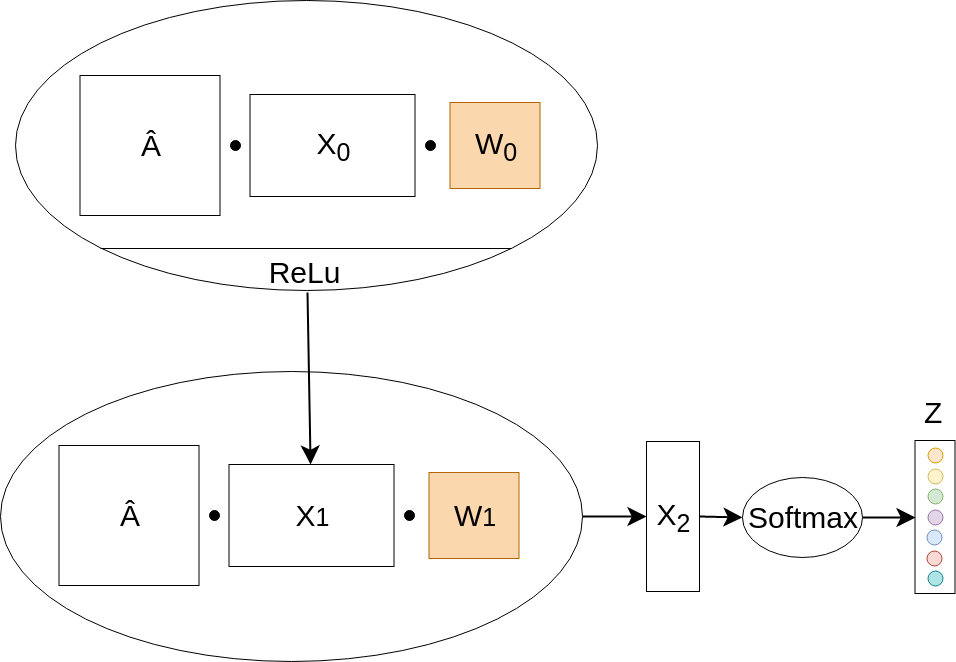
\includegraphics[width=0.75\linewidth]{media/model_right.png}
  
  \caption{Two-Layer Graph Convolution Network. This is the model used for all experiments in this paper.}
  \label{fig:model}
\end{figure}

In the forward pass, the first layer takes as input a matrix $x_{0}$ that contains the features for each node in the graph. The dot product of this matrix with the \textit{normalized adjacency matrix} $\hat{A}$ and the weight matrix $w_{0}$ is passed through the \textit{RelU} activation function and then used as the input for the next layer. In layer 2, the dot product of $x_{1}$ (output from layer 1) with the same \textit{normalized adjacency matrix} $\hat{A}$ and a second matrix of weights $w_{1}$. Finally, the matrix produced by the second layer is passed through a \textit{softmax} layer to generate a score for each class.

\subsection{Datasets}

We reproduced the experiments in~\cite{Kipf2016} on the Cora, Citesser and Pubmed datasets. In all three datasets, nodes are papers (documents) and the edges are citation links. Table~\ref{tab:datasets} shows the number of nodes, classes, features, and trainable nodes for each dataset. While training is only performed on nodes that have labels, recall in Equation \ref{eq:model} that the adjacency matrix is used in each convolutional layer. During training, all but twenty labels per class are removed from the graph. 

\begin {table}[ht!]
  \begin{center}
    \begin{tabular}{|c|c|c|c|c|}
    \hline
    Dataset  & Nodes  & Classes & Features & Trainable nodes\\
    \hline 
    Cora     & 2,708  & 7       & 1,433    & 140 \\ 
    Citeseer & 3,327  & 6       & 3,703    & 120  \\  
    Pubmed   & 19,717 & 3       & 500      & 60   \\
    \hline
    \end{tabular}
  \end{center}
\caption {Properties for each of the datasets. Features are bag-of-words for each paper (node in the graph).} \label{tab:datasets} 
\end{table}

\subsection{Experiment 1}

We reproduced the authors' experiments with the hyperparameters presented in Table \ref{tab:hyperparameters1}.

\begin {table}[ht!]
  \begin{center}
    \begin{tabular}{|c|c|}
    \hline
    Learning rate     & 0.01 \\ 
    Epochs            & 200  \\ 
    Optimization      & ADAM \\
    Drop out          & 0.5   \\
    Weight Decay      & 0.0005 \\
    Regularization    & L2    \\
    Hidden Features   & 16    \\
    \hline
    \end{tabular}
  \end{center}
\caption {Hyperparameters used in Experiment 1. These are extracted directly from~\cite{Kipf2016}.} \label{tab:hyperparameters1} 
\end{table}

 The results for this experiment are described in Table \ref{tab:results1}.

\begin {table}[ht!]
  \begin{center}
    \begin{tabular}{|c|c|c|c|c|}
    \hline
    Dataset    &  Training Accuracy & Validation Accuracy & Testing Accuracy & \cite{Kipf2016} Testing Accuracy \\ \hline
    Cora          & 99.43 \% & 73.80 \%  & 81.05 \% & 81.50 \% \\ 
    Citesser      & 94.92 \% & 62.84 \%  & 71.70 \% & 70.30 \% \\
    Pubmed        & 98.67 \% & 76.28 \%  & 80.00 \% & 79.00 \% \\
    \hline
    \end{tabular}
  \end{center}
\caption {Comparison between results reported in~\cite{Kipf2016} and results from our reproduction of their model. As expected, our results are very similar to those reported by Kipf and Welling.} \label{tab:results1} 
\end{table}

From the results in Table \ref{tab:results1} for Validation Accuracy, it is clear that overfitting is a problem with GCNs. We believe this is a result of the dramatic difference in size between the training and validation sets. Just 5\% of the nodes are labeled, so its understandable that the model has trouble generalizing for a large validation set. 

\subsection{Experiment 2}
For our second experiment, we trained the Cora dataset and fine-tuned our own hyperparameters. Our best results come from using the hyperparameters shown in Table \ref{tab:hyperparameters2}.

\begin {table}[ht!]
  \begin{center}
    \begin{tabular}{|c|c|}
    \hline
    Learning rate     & 0.012 \\ 
    Epochs            & 200  \\ 
    Optimization      & ADAM \\
    Drop out          & 0.64   \\
    Weight Decay      & 0.0006 \\
    Regularization    & L2    \\
    Hidden Features   & 102   \\
    \hline
    \end{tabular}
  \end{center}
\caption {Final hyperparameters found by Experiment 2.} \label{tab:hyperparameters2} 
\end{table}

The results for Experiment 2 are presented in Table~\ref{tab:results2}.

\begin {table}[ht!]
  \begin{center}
    \begin{tabular}{|c|c|c|c|}
    \hline
    Dataset    &  Training Accuracy & Validation Accuracy & Testing Accuracy\\ \hline
    Cora          & 98.57 \% & 75.80 \%  & 81.80 \% \\ 
    Citesser      & 100.00 \%& 67.20 \%  & 71.20 \% \\
    Pubmed        & 100.00 \%& 77.80 \%  & 79.30 \% \\
    \hline
    \end{tabular}
  \end{center}
\caption {Results from Experiment 2.} \label{tab:results2} 
\end{table}

The hyperparameters we found through Experiment 2 result in slightly worse Validation Accuracies than in Experiment 2. Overfitting is also slightly worse in Experiment 2. Overall, however, accuracies between the two experiments follow the same trends and small differences are probably a result of the extent to which Kipf and Welling fine-tuned their parameters. 

\subsection{Loss}

The loss function for this experiment is the standard multi-class \textit{cross-entropy loss}:

\begin{equation}
  \label{loss}
  \mathcal{L} = - \sum_{l \in \mathcal{Y}_{L}} \sum_{f=1}^{F} Y_{lf}lnZ_{lf}  
\end{equation}

Y is the ground truth and Z is the prediction (output of the model). Tables~\ref{tab:loss1} and~\ref{tab:loss2} show the loss for the model trained with the hyperparameters shown in Table~\ref{tab:hyperparameters2}.

\begin {table}[ht]
\parbox{.45\linewidth}{
\begin{center}
  \begin{tabular}{|c|c|}
  \hline
  Dataset       &  Loss\\ \hline
  Cora          & 0.7964997291564941 \\ 
  Citesser      & 0.9455778002738953 \\
  Pubmed        & 0.5608009696006775 \\
  \hline
  \end{tabular}
\end{center}
\caption {Loss from Experiment 1.} \label{tab:loss1} 
}
\hfill
\parbox{.45\linewidth}{
\begin{center}
  \begin{tabular}{|c|c|}
  \hline
  Dataset       &  Loss\\ \hline
  Cora          & 0.7033339738845825 \\ 
  Citesser      & 0.9455778002738953 \\
  Pubmed        & 0.5608009696006775 \\
  \hline
  \end{tabular}
\end{center}
\caption {Loss from Experiment 2.} \label{tab:loss2} 
}
\end{table}

Kipf and Welling do not provide any results for loss in~\cite{Kipf2016}.